\documentclass[../ManualeSviluppatore_v1.0.0.tex]{subfiles}

\begin{document}

\section{Configurazione dell'Ambiente di Lavoro}
	Per l'utilizzo del software è necessaria l'installazione della piattaforma Node.js, del node package manager (npm) e del sistema software di controllo di versione distribuito Git.
	\subsection{Installazione di Git}
		\subsubsection{Ubuntu 16.04 LTS}
			Eseguire da terminale il seguente comando:
				\begin{center}
					\texttt{\$ apt install git}
				\end{center}	
		\subsubsection{Mac OSX}
			Eseguire da terminale il seguente comando, dopo aver installato \gls{Homebrew} (\url{http://brew.sh/}):
				\begin{center}
					\texttt{\$ brew install git}
				\end{center}
		\subsubsection{Windows}
			Scaricare l'eseguibile di msysGit dal sito: \url{http://msysgit.github.io/} e procedere con l'installazione.
	\subsection{Installazione di Node.js}
		Scaricare l'installer corretto in base al proprio sistema operativo, reperibile alla pagina ufficiale di download di Node.js (\url{https://nodejs.org/it/download/}). Procedere dunque con l'installazione di Node.js.
	\subsection{Download dei file da GitHub}
		Eseguire da terminale il seguente comando:
			\begin{center}
				\texttt{\$ git clone ----recursive-submodules https://github.com/Kern3lP4nic/AtAVi}
			\end{center}
	\subsection{Installazione Dipendenze Back-End}
		Aprire il terminale nella cartella con il seguente percorso: *repo scaricata al punto 5.3*/back-end/Skill ed eseguire il seguente comando:
			\begin{center}
				\texttt{\$ npm install}
			\end{center}
	\subsection{Installazione Dipendenze per eseguire i Test}
		Tenendo come riferimento il percorso descritto al punto precedente, eseguire il seguente comando:
			\begin{center}
				\texttt{\$ npm install ----only=dev}
			\end{center}
	\subsection{Esecuzione dei Test}
		Tenendo come riferimento il percorso descritto al punto precedente, eseguire il seguente comando:
			\begin{center}
				\texttt{\$ mocha test}
			\end{center}
	\subsection{Configurazione chiavi di autenticazione}
		\subsubsection{Generare il \gls{token} di Slack}
			\begin{enumerate}
				\item Prima di tutto è necessario possedere un account Slack. Nel caso non fosse ancora stato fatto, è possibile procedere con la creazione di un utente all'indirizzo: \url{https://slack.com};
				\item Una volta effettuato l'accesso a Slack è necessario creare un team. Successivamente bisogna recarsi all'indirizzo: \url{https://api.slack.com/slack-apps}, premere in pulsante \textbf{Create a Slack app}, fornire il nome dell'app che si vuole realizzare e selezionare il proprio team di lavoro. A questo punto l'app sarà stata creata con successo;
				\begin{figure}[!h]
					\centering
					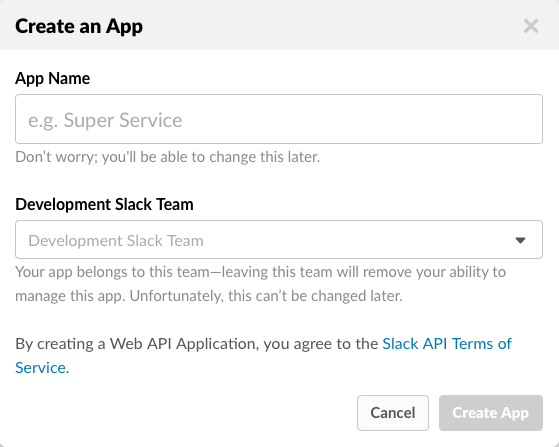
\includegraphics[scale=0.54]{Screenshot/CreateSlack.png}
					\caption{Creazione di una Slack app}
				\end{figure}
				\item Premere il pulsante per recarsi alla pagina di assegnazione dei permessi, \textbf{OAuth \& Permissions};
				\newpage
				\item Una volta giunti qui, nella sezione \textbf{Permission Scopes}, selezionare i seguenti permessi:
					\begin{itemize}
					\item Administer the team
					\item Post to specific channels in Slack
					\item Access information about user’s public channels
					\item Modify your public channels
					\item Send messages as *Nome App*
					\item Access information about your team
					\item Access your team's profile information
					\end{itemize}
				\begin{figure}[!h]
					\centering
					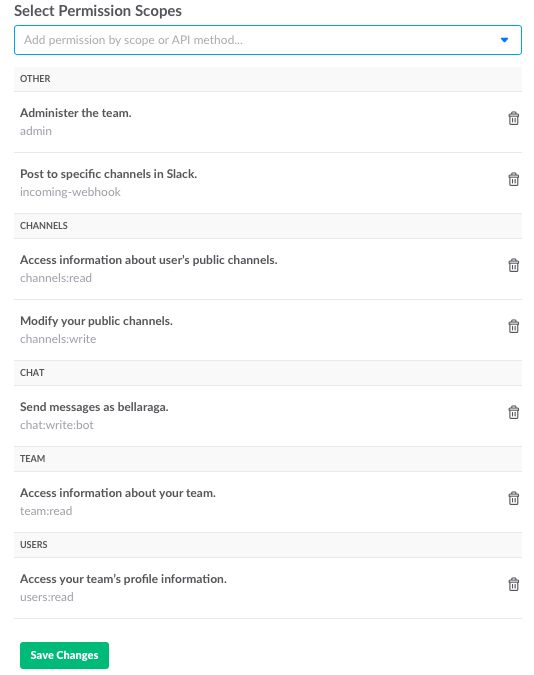
\includegraphics[scale=0.54]{Screenshot/PermessiSlack.png}
					\caption{Permessi dell'app di Slack}
				\end{figure}
				\item Una volta assegnati i permessi, nella sezione \textbf{OAuth Tokens \& Redirect URLs}, premere il pulsante \textbf{Install App to Team} e selezionare il team ed un canale afferente ad esso sul quale poter andare a pubblicare i messaggi;
				\newline
				\textbf{N}.\textbf{B}.: Con i permessi sopra assegnati, una volta installata l'app su un canale, sarà possibile pubblicare in tutti i canali associati al team specificato;
				\item Finalmente, sotto la voce \textbf{OAuth Access Token} verrà generato il token che dovrà essere copiato alla voce \textbf{tokenSlack} all'interno di un file da creare chiamandolo \textbf{config.json} situandolo nella cartella: *repo scaricata al punto 5.3*/back-end/ Skill/LambdaSkill/Actions/ActionsModules/MessageSlack/Slack, secondo la seguente struttura:
				\begin{lstlisting}[language=json,firstnumber=1]
{
	"tokenSlack":""
}
				\end{lstlisting}
				\begin{figure}[!h]
					\centering
					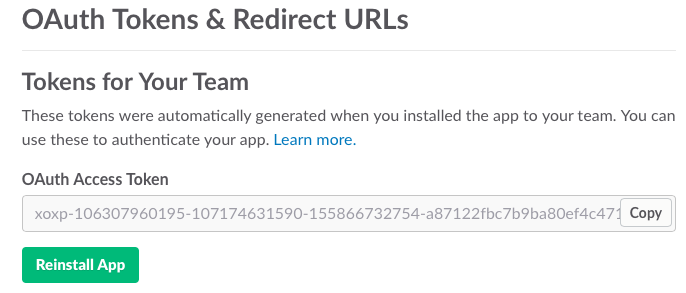
\includegraphics[scale=0.54]{Screenshot/OAuth.png}
					\caption{OAuth Access Token}
				\end{figure}
			\end{enumerate}
		\subsubsection{Chiavi d'accesso Amazon}
			\begin{enumerate}
			\item Prima di tutto è necessario possedere un account Amazon. Nel caso non fosse ancora stato fatto, è possibile procedere con la creazione di un utente all'indirizzo: \url{https://www.amazon.it};
			\item Dopo aver effettuato il Login, recarsi alla pagina della console amministrativa di Amazon all'indirizzo: \url{https://console.aws.amazon.com/console/home};
			\item Recarsi nella sottosezione \textbf{IAM} presente nella sezione \textbf{Security, Identity \& Compliance};
			\item Recarsi alla sezione \textbf{Create individual IAM users}, premere il pulsante \textbf{Manage Users} e successivamente \textbf{Add user};
			\begin{figure}[!h]
				\centering
				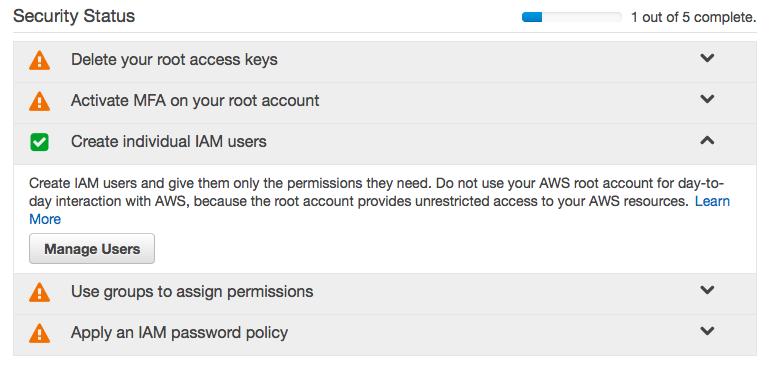
\includegraphics[scale=0.45]{Screenshot/IAMusers.png}
				\caption{Create individual IAM users}
			\end{figure}
			\item Compilare il campo \textbf{User name} e spuntare entrambi i flag della sezione \textbf{Access type}, poi premere il pulsante \textbf{Next: Permissions};
			\item Nella sezione \textbf{Attach existing policies directly} spuntare i flag corrispondenti a:
				\begin{itemize}
					\item AmazonDynamoDBFullAccess
					\item AmazonDynamoDBFullAccesswithDataPipeline
					\item AmazonAPIGatewayAdministrator
					\item AmazonAPIGatewayInvokeFullAccess
				\end{itemize}
			\begin{figure}[!h]
				\centering
				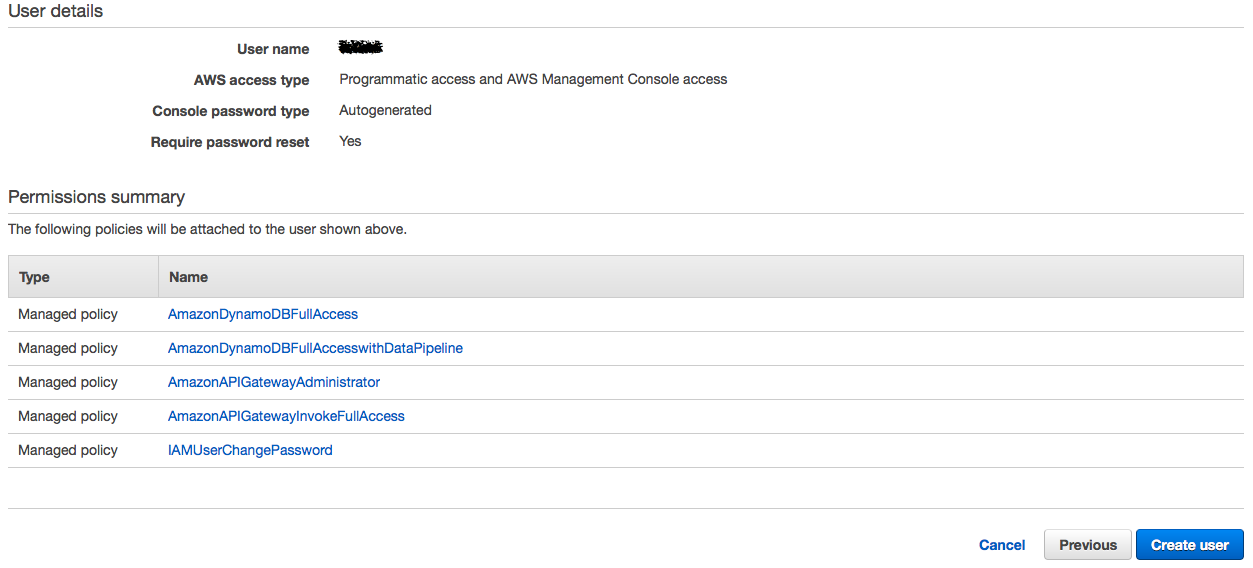
\includegraphics[width=\textwidth]{Screenshot/Usersdetails.png}
				\caption{User Details}
			\end{figure}
			\item Premere il pulsante \textbf{Next: Review} ed infine \textbf{Create user}. Se la creazione è avvenuta con successo, sarà reso disponibile il pulsante \textbf{Download .csv} che permetterà di scaricare un file contenente i dati sensibili da inserire all'interno di un file da creare, denominato \textbf{config.json} situato nella cartella: *repo scaricata al punto 5.3*/back-end/ Skill/LambdaSkill/QuestionService/DatabaseInteraction, secondo la seguente struttura:
			\begin{lstlisting}[language=json,firstnumber=1]
{
    "accessKeyId":"",
    "secretAccessKey":""
}
			\end{lstlisting}
		\end{enumerate}
	\newpage
	\subsection{Caricare le funzioni su AWS Lambda}
		\begin{enumerate}
			\item Per ognuna delle seguenti cartelle seguire pedissequamente i punti sucessivi:
				\begin{itemize}
				\item ManageFirm
				\item ManageSlack
				\item LambdaManageAdministrators
				\item LambdaManageAdmin
				\item refreshtoken
				\item ManageQuestion
				\item AmazonRefreshToken
				\item AmazonGetCode
				\end{itemize}
			\begin{comment}
			Clonare le seguenti repository da GitLab con il seguente comando da terminale:
			\begin{center}
				\texttt{\$ clone *url repository* ----recursive-submodules}
			\end{center}
			utilizzando come url i seguenti:
			\begin{itemize}
				\item \url{https://gitlab.com/kern3lp4nic/ManageFirm};
				\item \url{https://gitlab.com/kern3lp4nic/ManageSlack};
				\item \url{https://gitlab.com/kern3lp4nic/LambdaManageAdministrators};
				\item \url{https://gitlab.com/kern3lp4nic/LambdaManageAdmin};
				\item \url{https://gitlab.com/kern3lp4nic/refreshtoken};
				\item \url{https://gitlab.com/kern3lp4nic/ManageQuestion};
				\item \url{https://gitlab.com/kern3lp4nic/AmazonRefreshToken};
				\item \url{https://gitlab.com/kern3lp4nic/AmazonGetCode}.
			\end{itemize}
			\end{comment}
			\item Con il terminale, posizionarsi all'interno delle repository elencate al punto precedente e, per ognuna di esse, eseguire il comando:
			\begin{center}
				\texttt{\$ npm install}
			\end{center}
			\item Dentro ogni repository precedentemente scaricata è presente un'altra repository denominata \textbf{DatabaseInteraction}. All'interno di questa è necessario creare il file \textbf{config.json}, il quale va compilato con i dati contenuti all'interno del file .csv scaricato nella sezione 5.7.2, secondo la seguente struttura:
			\begin{lstlisting}[language=json,firstnumber=1]
{
	"accessKeyId":"",
	"secretAccessKey":""
}
			\end{lstlisting}
			\item Ora è necessario comprimere il contenuto di ogni repository.
			\newline
			\textbf{N}.\textbf{B}.: Non bisogna comprimere l'intera cartella, ma solo il suo contenuto. Il nome del file .zip creato deve corrispondere con il nome della cartella;
			\item A questo punto è necessario recarsi sul sito \url{https://console.aws.amazon.com/lambda/home?region=us-east-1#/functions?display=list}, premere il pulsante \textbf{Create a Lambda function} e successivamente premere il pulsante \textbf{avanti};
			\newpage
			\item In questa pagina è necessario inserire il nome preciso del file .zip creato in \textbf{Name}, una descrizione facoltativa in \textbf{Description}, in \textbf{Runtime} selezionare Node.js 6.10 ed infine in \textbf{Code entry type} sotto la sezione \textbf{Lambda function code}, dal menù a comparsa selezionare \textbf{upload a .ZIP file}, premere il tasto \textbf{Upload} e selezionare il corretto file compresso precedentemente creato
			\begin{figure}[!h]
				\centering
				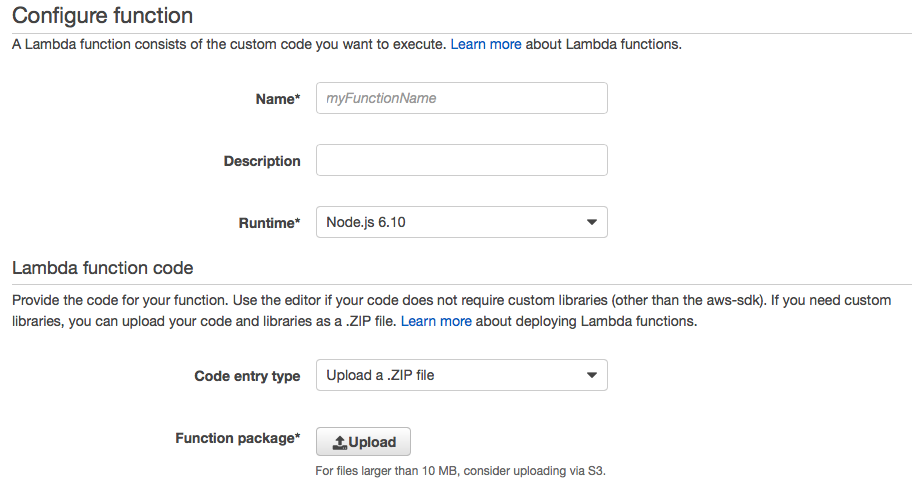
\includegraphics[width=\textwidth]{Screenshot/LambdaCreate.png}
				\caption{Create a New Lambda Function}
			\end{figure}
			\item Ripetere dal punto 3 per ogni file di tipo .zip creato. 
		\end{enumerate}
	\newpage
	\subsection{Importare impostazioni APIGateway}
		Collegarsi al sito \url{https://console.aws.amazon.com/apigateway/home}, premere il pulsante \textbf{Create API}, selezionare la voce \textbf{Import from Swagger}, premere il pulsante \textbf{Select Swagger File} e caricare i file \textbf{GuestHome\_v1.0.0.yaml} e \textbf{Administrationv\_1.0.0.yaml} situato nella directory principale della repository di \atavi\ e successivamente cliccare il pulsante \textbf{Import}.
		\begin{figure}[!h]
			\centering
			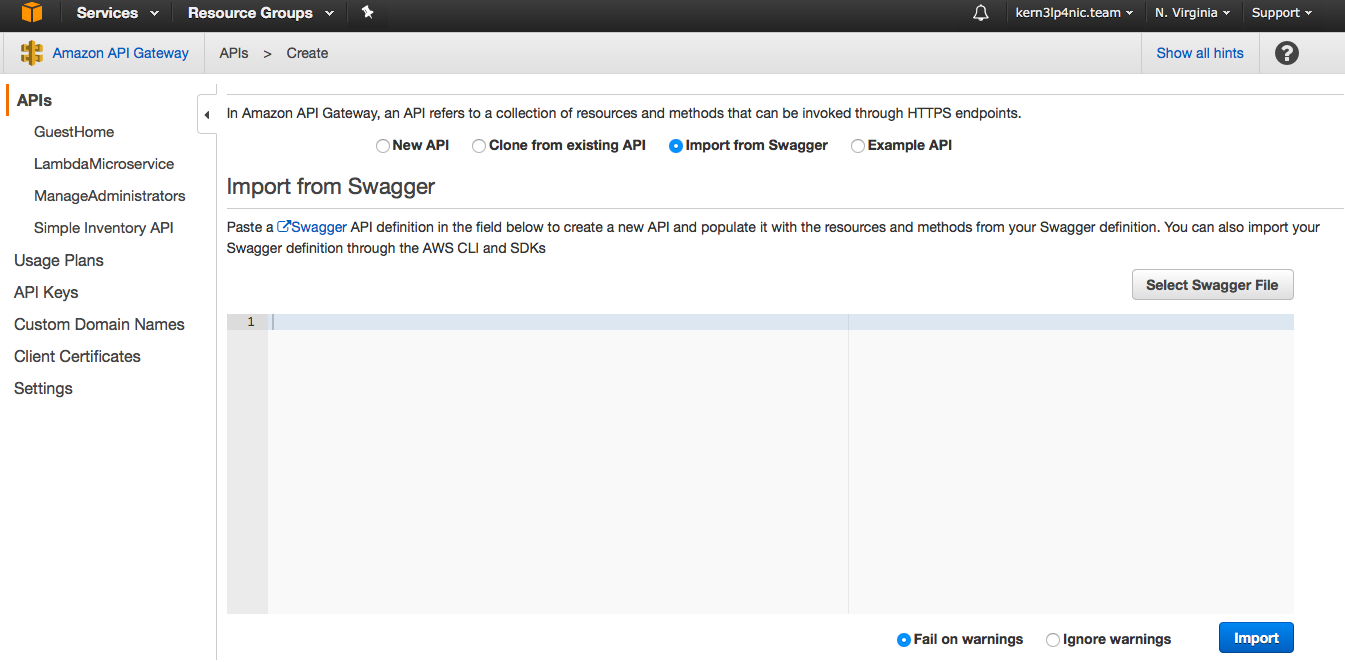
\includegraphics[width=\textwidth]{Screenshot/ImportSwagger.png}
			\caption{Import from Swagger}
		\end{figure}
	\subsection{Caricare tabelle su DynamoDB}
		\begin{enumerate}
		\item Collegarsi al sito \url{https://console.aws.amazon.com/dynamodb/home} e selezionare la voce \textbf{Tables} dal menù a sinistra;
		\item Per creare le tabelle premere il pulsante \textbf{Create table} e, nella creazione inserire i seguenti dati:
			\begin{longtable}[c] { >{\centering\arraybackslash}p{5cm} >{\centering\arraybackslash}p{5cm} }
				\toprule
				{\textbf{Table name}} & {\textbf{Primary key}} \\
				\midrule
				admin & username (String) \\
		 		\addlinespace[0.3em]
				\midrule
				databasetest & name (String) \\
		 		\addlinespace[0.3em]
		 		\midrule
				firm & name (String) \\
		 		\addlinespace[0.3em]
		 		\midrule
				firms & name (String) \\
		 		\addlinespace[0.3em]
		 		\midrule
				guest\_interaction & sessionId (String) \\
		 		\addlinespace[0.3em]
		 		\midrule
				interlocutor & id\_slack (String) \\
		 		\addlinespace[0.3em]
		 		\midrule
				question & id (Number) \\
		 		\addlinespace[0.3em]
		 		\midrule
				ServiceTest & name (String) \\
		 		\addlinespace[0.3em]
		 		\midrule
				test & id (Number) \\
		 		\addlinespace[0.3em]
		 		\bottomrule
		 		\caption{Corrispondenza fra Nome della Tabella e Chiave Primaria}
		 	\end{longtable}
		\item Nella repository principale contenente il progetto \atavi\ è disponibile la directory \textbf{Database Dump} ed al suo interno, sono disponibili dei file .json contenenti un amministratore SuperAdmin per accedere all'area amministrativa e alcune domande principali. I file sono utilizzabili come template per la creazione di tabelle all'interno di DynamoDB.
	\end{enumerate}
	
	\subsection{Configurazione Alexa Voice Service}
		\begin{enumerate}
			\item Effettuare il Login con le credenziali sviluppatore Amazon al seguente link: \url{https://developer.amazon.com/home.html}, selezionare la voce \textbf{Alexa} nella barra in alto e successivamente \textbf{Alexa Voice Service};
			\item In questa nuova pagina premere il pulsante \textbf{Register a Product} in alto a destra e selezionare \textbf{Application} dal menù che comparirà a ridosso del bottone
				\begin{figure}[!h]
					\centering
					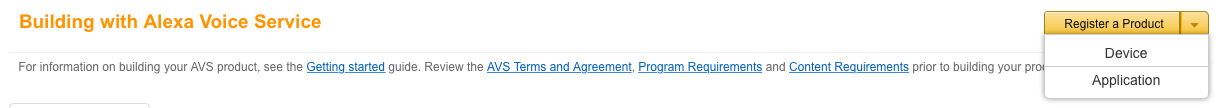
\includegraphics[width=\textwidth]{Screenshot/AVS/Application.png}
					\caption{Building with Alexa Voice Service}
				\end{figure}
			\item In \textbf{Application Type Info} compilare tutti i campi richiesti, in \textbf{Security Profile}, premere il pulsante \textbf{Select Security Profile} e, nel menù che appare, selezionare \textbf{Create a new profile}, compilare i campi richiesti e premere sul pulsante \textbf{Next} in basso a destra. Ora non resta che compilare anche i campi nella sezione \textbf{Application Details};
			\item Ora è necessario tornare alla sezione \textbf{Security Profile} ed entrare nella sottosezione \textbf{Web Settings}, inserire l'url corretto dell'applicazione \atavi nei campi \textbf{Allowed Origins} e \textbf{Allowed Return URLs}
				\begin{figure}[!h]
					\centering
					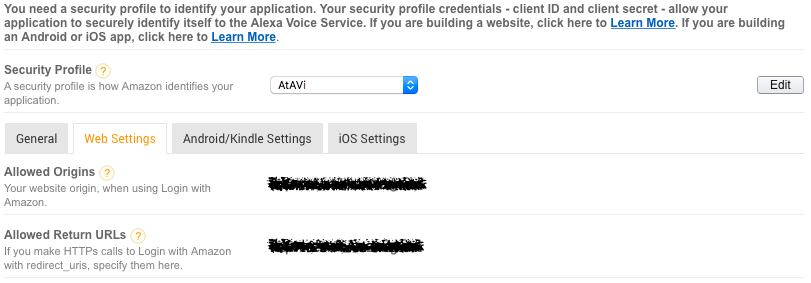
\includegraphics[width=\textwidth]{Screenshot/AVS/SecurityProfile.png}
					\caption{Security Profile \- Web Settings}
				\end{figure}
		\end{enumerate}
	\subsection{Configurazione Alexa Skills Kit}
		\begin{enumerate}
			\item Effettuare il Login con le credenziali sviluppatore Amazon al seguente link: \url{https://developer.amazon.com/home.html}, selezionare la voce \textbf{Alexa} nella barra in alto e successivamente \textbf{Alexa Skills Kit};
			\item Premere sul pulsante \textbf{Add a New Skill} e compilare le sezioni con i seguenti dati:
				\begin{itemize}
				\item Skill Information
					\begin{figure}[!h]
						\centering
						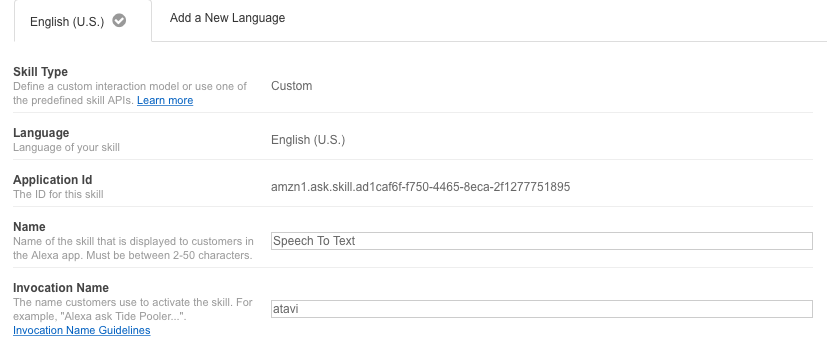
\includegraphics[width=\textwidth]{Screenshot/ASK/SkillInformation.png}
						\caption{Skill Information}
					\end{figure}
				\item Interaction Model
					\begin{figure}[!h]
						\centering
						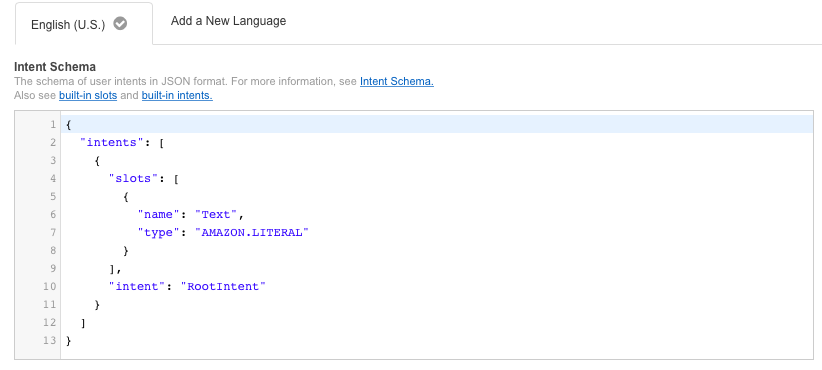
\includegraphics[width=\textwidth]{Screenshot/ASK/InteractionModel1.png}
						\caption{Intent Schema}
					\end{figure}
					\begin{figure}[!h]
						\centering
						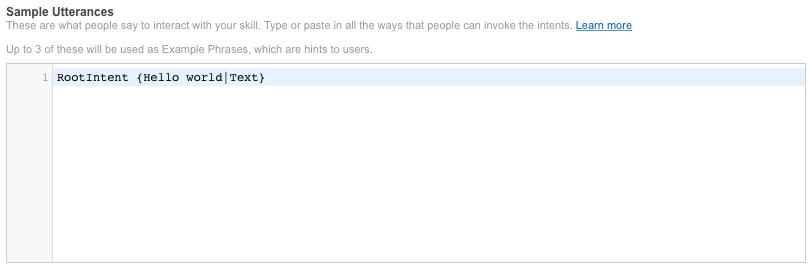
\includegraphics[width=\textwidth]{Screenshot/ASK/InteractionModel2.png}
						\caption{Sample Utterances}
					\end{figure}
				\newpage
				\item Configuration
					\begin{figure}[!h]
						\centering
						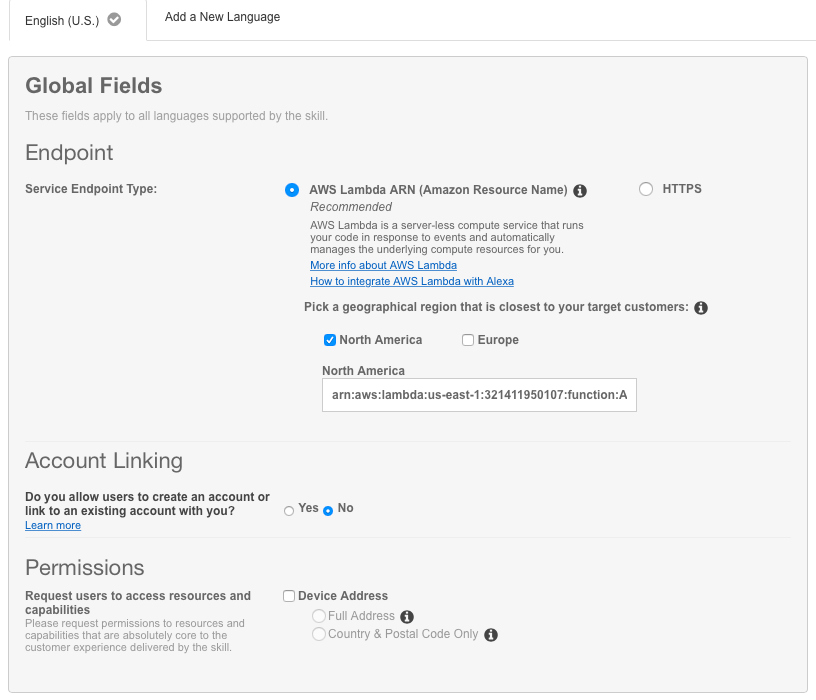
\includegraphics[width=\textwidth]{Screenshot/ASK/Configuration.png}
						\caption{Configuration}
					\end{figure}
				\item Test: abilitare la possibilità di effettuare test nel proprio account.
				\newpage
				\item Privacy \& Compliance
					\begin{figure}[!h]
						\centering
						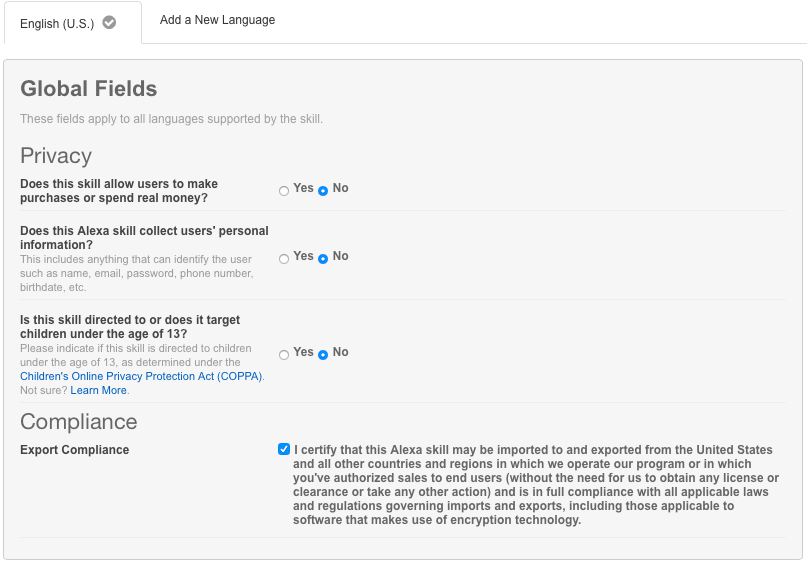
\includegraphics[width=\textwidth]{Screenshot/ASK/PrivacyCompliance.png}
						\caption{Privacy \& Compliance}
					\end{figure}
				\end{itemize}
		\end{enumerate}
		%TO DO
\end{document}